% =====================================================================
% Axona Architecture
% David A. Smith, Axona.net
%
% Compile with:  tectonic Axona-Architecture.tex
% Requires: tufte-latex, tikz, pgfplots, xcolor, booktabs, microtype
% (tectonic auto-fetches all of these; no system TeX needed)
% =====================================================================

\documentclass[nobib]{tufte-handout}

\usepackage[utf8]{inputenc}
\usepackage{amsmath}
\usepackage{amssymb}
\usepackage{tikz}
\usepackage{pgfplots}
\pgfplotsset{compat=1.18}
\usetikzlibrary{positioning, calc, arrows.meta, shapes.geometric}
\usepackage{xcolor}
\usepackage{booktabs}
\usepackage{microtype}
\usepackage{fancyhdr}
\usepackage{etoolbox}
\usepackage{needspace}
\usepackage{listings}

\lstdefinestyle{axonacode}{
  basicstyle=\ttfamily\fontsize{7.5}{9}\selectfont,
  breaklines=true,
  breakatwhitespace=false,
  columns=fullflexible,
  keepspaces=true,
  showstringspaces=false,
  frame=none,
  xleftmargin=0pt,
  aboveskip=0.4em,
  belowskip=0.4em,
}
\lstset{style=axonacode}

\pretocmd{\section}{\needspace{6\baselineskip}}{}{}
\pretocmd{\subsection}{\needspace{4\baselineskip}}{}{}

% Long \texttt{} literals + tufte's narrow measure: let LaTeX stretch a
% little rather than overflow into the margin.
\setlength{\emergencystretch}{3em}

\definecolor{rust}{RGB}{185,78,54}
\definecolor{rustsoft}{RGB}{212,168,150}
\definecolor{inkmuted}{RGB}{102,102,102}
\definecolor{codebg}{RGB}{240,236,223}

\setcounter{secnumdepth}{1}
\renewcommand{\thesection}{\Roman{section}}

\title{Axona Architecture}
\author[David A. Smith]{David A. Smith \\[0.3em] \emph{\small Axona.net}}
\date{}

\begin{document}

\fancypagestyle{ndhtplain}{%
  \fancyhf{}%
  \renewcommand{\headrulewidth}{0pt}%
  \fancyfoot[C]{\thepage}%
}

% --------------------------------------------------------------------
% Title page
% --------------------------------------------------------------------
\thispagestyle{empty}
\null\vfill
\begin{center}
{\fontsize{48}{52}\selectfont \textsc{Axona}\par}
\vspace{0.6em}
{\Large\itshape Architecture\par}
\vspace{4em}
{\large David A.~Smith\par}
{\itshape\small Axona.net\par}
\vspace{2em}
{\small An Axona Architecture Note \quad v0.9.0 \quad 2026-07-01\par}
{\footnotesize\itshape describes the kernel 4.x line (routing-only axonic pub/sub)\par}
\end{center}
\vfill
\null
\newpage

% --------------------------------------------------------------------
% Mission epigraph page
% --------------------------------------------------------------------
\thispagestyle{empty}
\null\vfill
\begin{flushright}
\itshape A protocol is the contract between layers that don't trust each other.\par
\end{flushright}
\vfill
\null\newpage

% --------------------------------------------------------------------
% Body opens with page numbers
% --------------------------------------------------------------------
\pagestyle{ndhtplain}
\thispagestyle{ndhtplain}
\setcounter{page}{1}

% --------------------------------------------------------------------
% Body epigraph
% --------------------------------------------------------------------
\begin{quote}
  \itshape What I cannot create, I do not understand.\\[0.3em]
  \normalfont\textsc{\footnotesize Richard Feynman} \,$\cdot$\, 1988
\end{quote}

\vspace{1em}

% =====================================================================
% I. THE SYSTEM IN ONE PAGE
% =====================================================================
\section{The System in One Page}

\newthought{Axona is a communication network with no center.} There is
no server that holds the messages, no company that runs the feed, no
database that could be subpoenaed, throttled, or turned off. Every
participant --- a browser tab, a phone, a headless relay process ---
is an equal \emph{peer}, and the peers together \emph{are} the
infrastructure. If you have read this paragraph, you already know the
hardest thing about Axona; everything else in this document is
mechanism.

Three ideas carry the whole design:

\begin{description}
\item[Everything has an address in one shared space.] Every peer and
every topic gets a 264-bit number. The first byte says \emph{where on
Earth} it belongs (one of 192 geographic cells); the rest is a
cryptographic hash nobody can choose. Because peers and topics live in
the \emph{same} address space, ``who should be responsible for this
topic?'' has a mechanical answer: \emph{whichever live peer's address
is closest to the topic's address.} No election, no registry, no
assignment --- proximity \emph{is} the appointment.

\item[Each topic grows a tree.] The closest peer to a topic's address
becomes its \emph{root}. Subscribers send their subscription toward the
topic's address; the network's routing delivers it to the root, which
seats them. When the root has more direct subscribers than it wants to
serve ($20$), it delegates batches of them to child relays --- so a
popular topic grows a shallow, bushy distribution tree
automatically.\sidenote{The tree is why we call the design
\emph{axonic}: like a neuron's axon, one cell body (the root) fans a
signal out through branches to many terminals (the subscribers), and
the branching grows only where there is something to reach.} A publish
is routed the same way, arrives at the root, and flows down the tree to
everyone. When the root disappears --- a laptop lid closes --- the next
closest peer, already holding a warm copy of the topic's history,
takes over.

\item[Authorship is a signature, not an account.] Every message can be
signed by an \emph{author key} that has nothing to do with where its
owner is or which device they used. Anyone can verify who wrote a
message; nobody can forge one; and the network itself never learns
where an author lives.
\end{description}

\begin{figure}[h]
\centering
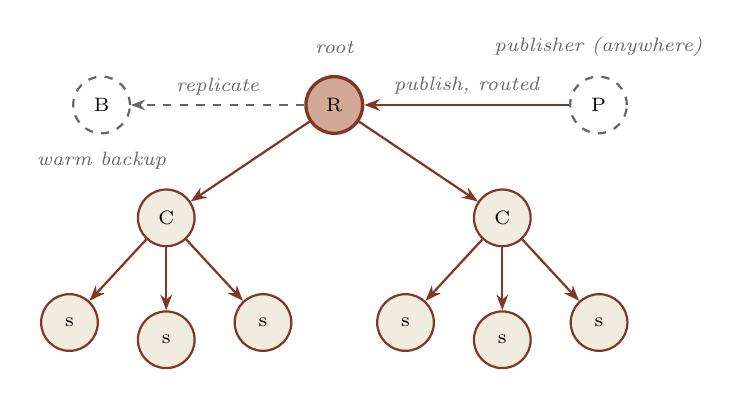
\begin{tikzpicture}[
  node distance=0.55cm and 0.7cm,
  peer/.style={draw=rust!70!black, fill=codebg, thick, circle,
    minimum size=0.72cm, font=\scriptsize, inner sep=1pt},
  root/.style={peer, fill=rustsoft, very thick},
  ghost/.style={peer, draw=inkmuted, dashed, fill=white},
  flow/.style={-{Stealth[length=2mm]}, rust!70!black, thick},
  soft/.style={-{Stealth[length=1.8mm]}, inkmuted, thin, dashed},
  lbl/.style={font=\scriptsize\itshape, inkmuted}
]
  % the root, closest to the topic id
  \node[root] (root) {R};
  \node[lbl, above=0.15 of root] {root};

  % child relays
  \node[peer, below left=0.9 and 1.6 of root] (c1) {C};
  \node[peer, below right=0.9 and 1.6 of root] (c2) {C};

  % subscribers
  \node[peer, below left=0.8 and 0.7 of c1] (s1) {s};
  \node[peer, below=0.8 of c1] (s2) {s};
  \node[peer, below right=0.8 and 0.7 of c1] (s3) {s};
  \node[peer, below left=0.8 and 0.7 of c2] (s4) {s};
  \node[peer, below=0.8 of c2] (s5) {s};
  \node[peer, below right=0.8 and 0.7 of c2] (s6) {s};

  % publisher, off to the side
  \node[ghost, right=2.6 of root] (pub) {P};
  \node[lbl, above=0.12 of pub] {publisher (anywhere)};

  \draw[flow] (pub) -- node[lbl, above, sloped] {publish, routed} (root);
  \draw[flow] (root) -- (c1);
  \draw[flow] (root) -- (c2);
  \draw[flow] (c1) -- (s1); \draw[flow] (c1) -- (s2); \draw[flow] (c1) -- (s3);
  \draw[flow] (c2) -- (s4); \draw[flow] (c2) -- (s5); \draw[flow] (c2) -- (s6);

  % backup cohort
  \node[ghost, left=2.2 of root] (b1) {B};
  \node[lbl, below=0.10 of b1] {warm backup};
  \draw[soft] (root) -- node[lbl, above, sloped] {replicate} (b1);
\end{tikzpicture}

\medskip
{\footnotesize\itshape One topic, one emergent tree. The root (R) is
simply the live peer closest to the topic's address. The publisher
routes its message toward that address; the root stamps and fans it
down through child relays (C) to subscribers (s); a warm backup (B)
stands by with a replicated copy of the history. Nothing in this
picture was configured --- every role is a consequence of address
proximity and load.\par}
\end{figure}

The rest of this document walks the same picture at increasing
magnification: the software layers that implement it (\S\,II--IV), the
routing fabric underneath it (\S\,V--VI), the pub/sub tree itself and
the life of one message through it (\S\,VII--IX), what happens when
things fail (\S\,X), and the transports, servers, wire format,
security model, and deployment that carry it in production
(\S\,XI--XVI).

% =====================================================================
% II. THE STACK
% =====================================================================
\section{The Stack}

\newthought{Axona ships as four repositories} that compose into one
running system. Each layer has a single
responsibility,\sidenote{The pattern is intentional. A peer's
business logic should never need to know the wire format; a bridge
should never need to know what topic a subscriber cares about; the
kernel should never need to know which application is using it. Every
interface in this document is a place where one layer was given the
right to be wrong about the layer below.} a single canonical version
identifier (\texttt{KERNEL\_VERSION}), and a contract surface narrow
enough to fit on a postcard.

\begin{description}
\item[\texttt{@axona/protocol} (kernel).] The pure-JS library. Owns
the DHT routing, the axonic pub/sub overlay, the cryptography, and the
transport contracts. No browser DOM, no Node-specific I/O, no
network code outside abstract transport classes. Runs identically in
browsers, in Node, in dht-sim's simulated network. This document
describes the kernel \textbf{4.x} line (v4.15.0 at this writing).

\item[\texttt{axona-peer} (browser application).] The reference
end-user app. Provides identity persistence, region selection,
WebRTC mesh formation, a chat-style UI for pub/sub. Imports the
kernel as a vendored copy under \texttt{vendor/axona-protocol/} so
the version that ran when the page was built is the version that
runs in the browser.

\item[\texttt{axona-bridge} (deployed server).] The signaling +
introducer service. Runs an embedded
\texttt{AxonaPeer} of its own (so it is a full DHT participant, not
just a relay), gates connecting peers behind a version handshake,
mints short-lived TURN credentials, relays WebRTC signaling between
browsers, and forwards Axona wire frames addressed to its own
embedded peer.

\item[\texttt{axona-relay} (headless supernode).] A Node process that
joins the mesh over \emph{real} WebRTC (a spec \texttt{RTCPeerConnection}
from \texttt{node-datachannel}) and runs the same kernel stack a browser
peer runs --- routing lookups, rooting pub/sub topics, hosting its
keyspace neighborhood, relaying signaling for others --- but with no
DOM, no public server, and no TURN minting. It is a strict
\emph{subset} of the bridge: it dials a bridge once for bootstrap,
then is a first-class peer. Running several relays strengthens
routing and pub/sub durability without any of them being an inbound
server.
\end{description}

\marginnote{A fifth repository, \texttt{dht-sim}, runs the kernel
against a simulated network for protocol research and regression
benchmarks. It is not part of the production stack but shares the
same \texttt{@axona/protocol} library; protocol changes are validated
against its 25{,}000-node batteries --- and, since the sim can shrink
the keyspace (\texttt{configureKeyspace}), against large-population
churn experiments the full 264-bit space would make prohibitively
slow. A hard-won methodology rule rides along: a single simulation
run's delivery percentage is noise; every claim requires five or more
seeds reported as mean\,$\pm$\,sd.}

Each component carries its own semver track because each
ships to a different audience: kernel changes need API-level
discipline; peer changes are user-visible UI; bridge and relay changes
are operational deploys. But they all share the same kernel version,
visible at runtime through \texttt{/healthz} (bridge), the
\texttt{welcome} frame (any peer connecting), and the version row in
the peer UI.

\begin{figure}[h]
\centering
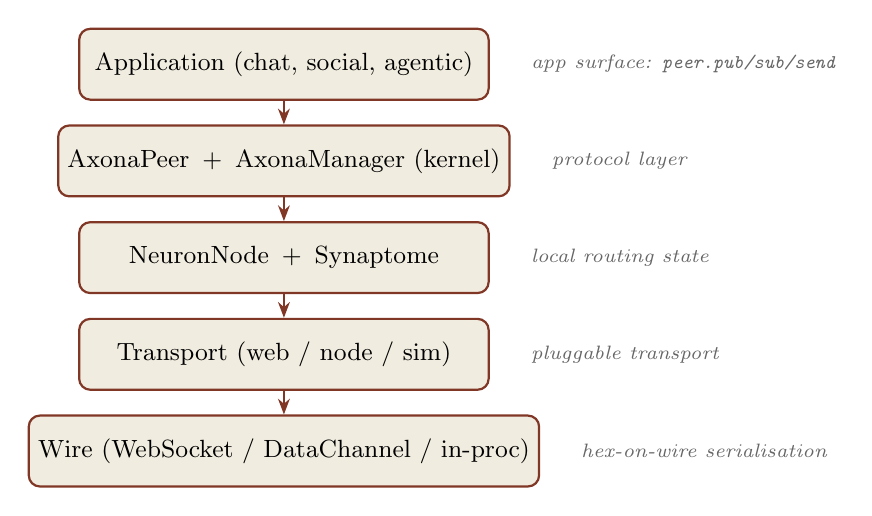
\begin{tikzpicture}[
  layer/.style={
    draw=rust!70!black, fill=codebg, thick, rounded corners,
    minimum width=5.2cm, minimum height=0.9cm, align=center,
    font=\small
  },
  conn/.style={-{Stealth[length=2mm]}, rust!70!black, thick},
  meta/.style={font=\scriptsize\itshape, inkmuted, align=left}
]
  \node[layer] (app)    {Application (chat, social, agentic)};
  \node[layer, below=0.3 of app] (peer)   {AxonaPeer \,+\, AxonaManager (kernel)};
  \node[layer, below=0.3 of peer] (node)   {NeuronNode \,+\, Synaptome};
  \node[layer, below=0.3 of node] (txp)    {Transport (web / node / sim)};
  \node[layer, below=0.3 of txp] (wire)   {Wire (WebSocket / DataChannel / in-proc)};

  \draw[conn] (app)  -- (peer);
  \draw[conn] (peer) -- (node);
  \draw[conn] (node) -- (txp);
  \draw[conn] (txp)  -- (wire);

  \node[meta, right=0.4 of app]   {app surface: \texttt{peer.pub/sub/send}};
  \node[meta, right=0.4 of peer]  {protocol layer};
  \node[meta, right=0.4 of node]  {local routing state};
  \node[meta, right=0.4 of txp]   {pluggable transport};
  \node[meta, right=0.4 of wire]  {hex-on-wire serialisation};
\end{tikzpicture}

\medskip
{\footnotesize\itshape Five layers in one peer. Every arrow is a
contract; every contract has a smoke-test suite.\par}
\end{figure}

% =====================================================================
% III. IDENTITY AND ADDRESSING
% =====================================================================
\section{Identity and Addressing}

\newthought{Axona keeps three concerns separate}, each with its own
primitive. \emph{Connection} is a node identity --- an Ed25519 keypair
whose public key yields a 264-bit \emph{Node ID}; it is ephemeral and
anchored to a region. \emph{Authorship} is an author identity --- a
location-free Ed25519 keypair whose public key \emph{is} the
\emph{Author ID} (the \texttt{signerPubkey} on the wire); it is durable
and a peer may hold several. \emph{Addressing} is the topic descriptor
and message ID, derived independently of either identity. The kernel
mints the two identities with separate factories
(\texttt{createNodeIdentity}, \texttt{createAuthorIdentity}); a publish
is signed per-call with an author, never with the connection key.

\newthought{The connection identity is a 264-bit identifier.} The
top 8 bits are a Google S2 cell prefix\sidenote{S2 projects the
sphere onto the six faces of a cube and partitions each face with an
equal-area quadratic transform. We bin each face into a
4\,$\times$\,8 grid (32 cells per face) --- ``S2 level 2.5,'' one bit
short of level 3's 8\,$\times$\,8 --- giving $6 \times 32 = 192$
cells, which fit in 8 bits with byte values 192--255 left reserved
for future system use. The quadratic projection keeps cell areas
within $\sim$1.7$\times$ of each other globally --- no polar
shrinkage --- and any standard S2 library can recompute our
prefixes.} computed from
the peer's latitude and longitude; the bottom 256 bits are the
SHA-256 of the peer's Ed25519 public key. A peer in London has an
ID starting with \texttt{0x44}; a peer in Virginia starts with
\texttt{0x89}. Two peers in the same region share a leading byte;
two random peers share only the bits their keys happen to share.

\marginnote{Each of the 192 cells carries exactly \emph{one}
human-readable name, so a region always presents the same label
(no location-dependent flip-flop). Where a cell straddles an ocean and a
landmass the land name wins; a multi-country cell takes its dominant city;
homogeneous cells (one country, open ocean) keep their name. A name is
usually unique to one code, though an area larger than one cell may span
adjacent codes. The kernel ships the canonical table and the
\texttt{regionName}/\texttt{regionCode}/\texttt{resolveRegion} helpers; the
\texttt{s2-region-visualizer} example renders all 192 ---
one name and the hex code each --- on a globe.}

\newthought{Inside the running system, an address is always a
\texttt{BigInt}; on the wire, always hex.} This is an enforced
invariant, not a convention.\sidenote{Kernel v4.14.0 made it
load-bearing: the one coercion gate, \texttt{asId()}, validates and
converts at every construction site (\texttt{DHTNode},
\texttt{Synapse}) and every wire-ingress point, so a routing object
\emph{cannot} hold a string address and internal code never asks
``string or bigint?'' The only sanctioned hex forms are a JSON wire
frame and an identity object's serialized \texttt{.id} /
\texttt{.authorId}.} The wire format is 66-character lowercase hex ---
the \textsc{only} representation that ever appears in JSON. The
conversion happens at exactly two kinds of place: when a frame is
serialised outbound, and at the \texttt{asId()} gate when one is
parsed inbound.

\textbf{An author identity carries no location.} Where the node ID
binds a key to a place, the Author ID is the bare Ed25519 public key
and nothing else --- no region byte, no coordinates. It is what a
reader recognises across sessions and devices; the same author key
signs from anywhere. Addressing never depends on it being co-located
with the publisher.

\textbf{Topic identifiers share the address space.} A topic is not a
bare string but a structured descriptor --- \texttt{\{region, owner?,
name, write\}} --- and its ID is \texttt{topicId =
regionByte\,||}\allowbreak\texttt{\,sha256(canonical(\{owner, name, write\}))}, so the top
byte is always a \emph{real}, routable S2 cell. The region comes from
one of two rules: an explicit \texttt{region} places the topic where
the application chooses (given as a region \emph{name or its code} ---
\texttt{'useast'} $\equiv$ \texttt{0x89} $\equiv$ \texttt{137}, all
normalising to the same region byte); if \texttt{region} is omitted, it defaults to
the \emph{publisher's own node region} --- the top byte of its node ID,
which is a real cell the publisher already occupies. The region is
\emph{never} derived from the author key: an Author ID has no region,
and hashing one into a region would dump every author's topics into a
single arbitrary cell, manufacturing a hot spot in whatever populated
region happened to fall closest. There is no synthetic publisher and no
\texttt{00} ``global'' bucket: every topic lands in a populated region,
and peers in that region are XOR-closest to it, which is what makes
regional pub/sub route naturally.\sidenote{Because the omitted-region
default is the \emph{publisher's} region, two co-located peers converge
on the same topic id without naming a region; cross-region discovery
names the region explicitly (typically alongside the owner and name).
The \texttt{write} field also folds into the hash: \texttt{open} lets
anyone publish (self-signed), \texttt{owner} restricts publishing to the
named owner Author ID. Because \texttt{owner} and \texttt{write} live
inside the signed descriptor, a host recomputes the topic ID and
enforces write authorisation statelessly --- see \S\,XIV.}

The Activation Potential (AP) routing formula, the topic-terminus
test, and the synaptome's stratum buckets all operate on this
one space. There is no separate ``topic ID space'' or ``peer ID
space''; they share addresses because they share routing --- and that
sharing is precisely what lets a topic's root be \emph{found} rather
than \emph{assigned}.

% =====================================================================
% IV. THE KERNEL: @axona/protocol
% =====================================================================
\section{The Kernel: \texttt{@axona/protocol}}

\newthought{The kernel is the protocol.} Everything else is its
clients. The directory structure mirrors the contract surface:

\begin{description}
\item[\texttt{src/contracts/}.] Abstract base classes: \texttt{Transport},
\texttt{DHT}, \texttt{DHTNode}, \texttt{BootstrapService},
\texttt{PersistenceAdapter}. These are the seams where alternate
implementations plug in. A custom transport (libp2p, QUIC, embedded)
extends \texttt{Transport}; a database-backed persistence
(IndexedDB, SQLite) extends \texttt{PersistenceAdapter}.

\item[\texttt{src/dht/}.] The active routing layer: \texttt{NeuronNode},
\texttt{Synapse}, \texttt{AxonaPeer}, \texttt{AxonaDomain},
\texttt{Subscription}. This is where the Axona routing logic lives,
and where the developer-facing API surface (\texttt{peer.pub},
\texttt{peer.sub}, \texttt{peer.ready}, \texttt{peer.lookup}) is
declared.

\item[\texttt{src/pubsub/}.] The pub/sub overlay: \texttt{AxonaManager}
(the axonic tree --- roles, the routed subscribe/publish handlers,
delegation, replication, the replay caches, the dedup index),
\texttt{post.js} (the topic descriptor + \texttt{resolveTopic} /
\texttt{deriveTopicId} derivation), \texttt{envelope.js} (signed
publish envelopes + write-policy checks), \texttt{kill.js} (signed
retractions), \texttt{metrics.js} (the derived metric-topic
convention), \texttt{authorClass.js} (agent-legibility attestations),
\texttt{ed25519.js} (Ed25519 binding for \texttt{crypto.subtle}).

\item[\texttt{src/transport/}.] Concrete transports:
\texttt{transport/web/} (browser: BridgeTransport over WebSocket +
WebRTCTransport over DataChannels), \texttt{transport/node/}
(server-side WebSocket), \texttt{transport/sim/} (in-process
simulation for dht-sim and tests). All implement the abstract
\texttt{Transport} contract identically. \texttt{handshake.js} owns
the version gate (\texttt{WIRE\_VERSION}, \texttt{KERNEL\_VERSION}).

\item[\texttt{src/utils/}.] Pure helpers: \texttt{hexid.js}
(the \texttt{asId} gate, BigInt$\leftrightarrow$hex conversions, XOR
distance, leading-zero count, the configurable keyspace profile),
\texttt{s2.js} (S2 cell computation), \texttt{region-names.js} (the
192-cell table and name helpers), JSON codec
(\texttt{transport/wire.js}).

\item[\texttt{src/identity/}.] Ed25519 keypair derivation +
persistence envelopes. Two factories, one per concern.
\texttt{createNodeIdentity(\{lat, lng\})} mints the \emph{connection}
identity: an ephemeral, location-anchored keypair returning
\texttt{\{id, pubkey, pubkeyHex, privateKey, region, \ldots\}}, where
\texttt{id} is the 264-bit Node ID.
\texttt{createAuthorIdentity(\{persistAs?, store?\})} mints the
\emph{authorship} identity: a location-free keypair returning
\texttt{\{authorId, pubkey, pubkeyHex, privateKey, \ldots\}} with no
\texttt{id} and no \texttt{region} --- \texttt{authorId} is the public
key, i.e.\ the \texttt{signerPubkey} on the wire. Persistence is an
option on the author factory, not a separate call.

\item[\texttt{std/}.] Optional application-layer conventions that ride
on the core API without touching the wire: \texttt{std/message}
(a common message shape so different apps render each other's posts),
\texttt{std/chunk} (chunked large-payload transfer under the
15\,KB reliable-delivery floor).
\end{description}

The whole kernel has zero runtime dependencies beyond the host
JavaScript environment (browser or Node 20+). No bundler, no
transpilation, no build step. The same source files run in the
browser via ES modules, in Node via direct \texttt{import}, and in
the simulator via the in-process transport.

% =====================================================================
% V. THE LOCAL NODE: NeuronNode + Synaptome
% =====================================================================
\section{The Local Node}

\newthought{Each peer's view of the network} lives in two data
structures on the \texttt{NeuronNode}: the \emph{synaptome} (its
outgoing connections) and the \emph{incoming synapse index} (peers
known to point at it). Both are keyed by 264-bit BigInt nodeId.

A \texttt{Synapse} is a routing edge --- it carries a peer ID, a
measured latency, a learned weight, a stratum (the XOR-distance
bucket), an inertia lock, and provenance (was this synapse added via
handshake, hop-cache, triadic introduction, or sponsor bootstrap?).
The synaptome is unbounded by design; the routing layer evicts
synapses through the \emph{Structural Survival Rule},\marginnote{The
rule, in one sentence: a synapse may only be pruned if at least one
other synapse with the same stratum exists. The effect: every
populated stratum keeps at least one live route, so the address
space stays globally navigable even after heavy decay.} which
guarantees navigability even under aggressive weight decay.

Routing decisions don't pick the XOR-closest synapse blindly. Each
candidate is scored by Activation Potential:

\[
AP_c \;=\; \frac{\Delta \text{Distance}_c}{L_c} \times (1 + w \cdot W_c)
\]

The first factor is progress velocity --- how much XOR distance the
hop closes per millisecond of measured latency. The second is a
mild boost for synapses that have historically led to fast lookups.
Weight only accrues on at-or-below-average-latency paths, so a
high-W synapse genuinely represents a fast route, not just a
frequently-used one. Two random hops with similar latency tie; the
one that's served us well before wins the tiebreak.

% =====================================================================
% VI. ROUTING
% =====================================================================
\section{Routing}

\newthought{Axona's routing is learning-adaptive.} It replaces
Kademlia's $k$-bucket array with a dynamic synaptome that adjusts
edge weights based on observed latency. The basic shape --- iterative
lookup, $\log_2(N)$ hop count --- is unchanged from Kademlia; what
changes is which peer you ask at each hop.

The five wire operations that drive Axona routing are:

\begin{description}
\setlength{\itemsep}{0pt}
\item[\texttt{lookup\_step} (req).] ``Here's a target. What's
your best next hop?'' The receiver evaluates AP across its
synaptome's progress candidates, returns the winning synapse + its
own routing state.

\item[\texttt{lookahead\_probe} (req).] ``If I forward to you for
target $T$, who would you forward to?'' A one-deep peek that lets
the caller compare expected hop costs across candidates before
committing.

\item[\texttt{find\_closest\_set} (req).] ``Give me your $K$
peers closest to this target.'' The K-closest harvester behind
\texttt{peer.findKClosest} --- used by the pub/sub layer to resolve a
topic's true neighborhood (root hints, replication cohorts, the
region-occupancy probe).

\item[\texttt{route\_msg} (req).] Generic routed-message
forwarder. This is the workhorse of the pub/sub layer: every
\texttt{pubsub:*} message (\S\,VII) rides it, greedily descending in
XOR distance toward a topic or peer id until it reaches the node
where no neighbor is closer --- the \emph{terminus}.

\item[\texttt{reinforce} (ntf).] ``This lookup succeeded; bump
the weight on the synapse I used.'' Fire-and-forget LTP signal
back along the path. Only flows when the lookup hit at-or-below
average latency for the path's region. On identity-binding
transports the handler is a no-op unless the \emph{target} synapse's
peer is currently bound (the B-3 gate: an unauthenticated
\texttt{reinforce} must not be able to refresh the eviction-inertia
of a stale or unverified entry and pin it in the table). Weight is
independently clamped to $\le 1.0$, so inertia is the only lever the
gate needs to close.
\marginnote{\emph{Residual, by design:} the gate keys on the
\emph{target} synapse being bound, not on the \emph{sender's}
identity --- so any bound peer can refresh the inertia of any other
bound peer's synapse. The blast radius is bounded to ``keep an
already-verified, live peer pinned slightly longer,'' which is
benign; binding the signal to the sender would add cost for no
attacker-relevant gain. Revisit only if reinforce ever carries
weight a sender could bias.}
\end{description}

Two structural-plasticity messages let the network rewire itself
without explicit instruction: \texttt{triadic\_introduce}
(``introduce me to your friend at $X$'') and \texttt{hop\_cache}
(``I've forwarded to $X$ several times; install a direct synapse to
$X$''). Both are fire-and-forget notifications that obey the
synaptome's admission rule (\texttt{\_addByVitality}).

\marginnote{The performance claim of Axona over Kademlia is roughly
40\% fewer wall-clock milliseconds per lookup at 25{,}000 nodes,
mostly from latency-weighted hop selection. The figure is documented
in the companion paper \emph{Axona: A Learning-Adaptive Distributed
Hash Table and Axonal Publish/Subscribe} (v0.4.01, 2026-05-23).}

\subsection{Synaptome Maintenance: Keeping the Near Neighborhood Complete}

\newthought{Greedy routing is only as good as the table is complete.}
A greedy walk toward a target descends in XOR distance until no neighbor
is closer --- a \emph{local minimum}. On a complete graph that minimum is
always the global one (the true target). On a real, \emph{incomplete}
synaptome (each peer holds $\sim$20 of $N$), a walk can dead-end at a
near-miss node instead. When a publisher and its subscribers dead-end at
\emph{different} near-miss nodes, they resolve different pub/sub roots and
never rendezvous --- the all-or-nothing delivery failure that dominates
under churn. The cure is table \emph{completeness}, in two co-equal parts
(classic Chord successors $+$ fingers, Kademlia closest-bucket $+$
distant-buckets):

\begin{description}
\setlength{\itemsep}{0pt}
\item[Successors (near quota).] Hold the $K_{\text{near}}{\approx}5$
XOR-closest peers. This clique completes the \emph{last mile}: the final
descent always lands on the true root. (Simulation: 4--6 is the knee;
more adds nothing.)
\item[Fingers (long range).] Hold $\sim$$\log(N)$ distant links --- one
per populated stratum --- so a walk can \emph{reach} the target's
neighborhood at all. These are maintained by the existing anneal and the
Structural Survival Rule; the simulation shows a perfect
successor set still fails to deliver if the long-range half is starved.
\end{description}

\newthought{Repair is local and cheap.} When a near-neighbor churns out,
its replacement is almost always a \emph{neighbor-of-neighbor} (the
``successor's successor''), found in a 1--2 hop local query --- never a
global lookup. The kernel runs a deterministic maintenance tick plus an
immediate pass on peer loss (\texttt{onPeerDied}); below quota it refills
from the nearest verified peer through the \emph{same} first-party
verification (\texttt{\_considerCandidate}) as any other synapse, bounded
to a few dials per pass. In sustained-churn simulation, an unmaintained
near-stratum erodes and delivery drifts down, while local refill holds it.

\marginnote{\emph{Eclipse note.} Dialing one's nearest peers is an
eclipse-sensitive surface, so refill admits \emph{only} first-party-verified
peers, never displaces a nearer honest peer for a farther attacker, and is
budget-bounded --- it adds no leverage beyond raw keyspace proximity. Making
that proximity costly to acquire is the job of costly identity (E-1,
memory-hard PoW), a \emph{pre-production} requirement; on a development
network with no adversary it is an accepted risk.}

\newthought{A second lesson from the churn experiments} shapes how a
node \emph{joins}: leaving is nearly free (neighbors route around a
dead node within a tick), but a \emph{newcomer} is invisible until its
neighbors' tables point at it --- and that reachability lives in
\emph{their} tables, not its own. Self-directed lookups do nothing for
it; what integrates a newcomer is \emph{inbound} traffic. The kernel
therefore treats directed integration --- a handful of packets routed
\emph{at} each newcomer --- as part of admission, which the simulation
showed heals reachability roughly 2.5$\times$ faster than blind
warm-up traffic of the same volume.

% =====================================================================
% VII. PUB/SUB: THE AXON TREE
% =====================================================================
\section{Pub/Sub: The Axon Tree}

\newthought{The 4.x line rebuilt pub/sub around a single idea:}
\emph{the tree is wherever routing says it is.} Earlier kernels used a
K-closest design --- publisher and subscriber each computed the $K$
peers nearest the topic and fanned out to all of them, hoping the sets
overlapped. On a real, gappy browser mesh they often did not: each
side ran its \emph{own} error-prone lookup, resolved \emph{different}
``closest'' nodes, and a publish landed on roots no subscriber was
attached to. Measured on the live testnet, that rendezvous failure ---
not bandwidth, not crypto --- was the dominant loss. The redesign
removes the independent lookups entirely.\sidenote{The cutover was a
clean break --- wire major 3\,$\to$\,4 --- because the two designs'
convergence semantics cannot interoperate: a 3.x peer fans out to
K roots that a 4.x network never consults. The full design rationale
is recorded in the \emph{Pubsub Axon Tree} note in
\texttt{axona-docs/architecture/}.}

\subsection{One root, found by routing}

Every pub/sub verb is a \emph{routed message toward the topic id}.
Whichever node the greedy walk terminates at --- the live peer
XOR-closest to the topic, the \emph{terminus} --- \emph{is} the root.
Root-ness is not elected, announced, or negotiated; it is the
by-product of the same routing that carries every other message, so
publisher and subscriber cannot disagree about where the root is any
more than two letters addressed identically can arrive at different
houses. On receiving a routed pub/sub message, a node makes a
four-way decision:

\begin{description}
\setlength{\itemsep}{0pt}
\item[\texttt{handle}.] I am the terminus (and, when the region lock
is enforced, in the topic's region): act as the root.
\item[\texttt{forward}.] I am not the terminus: pass it along the
greedy walk.
\item[\texttt{reroute}.] The message was aimed at a waypoint that is
me, but I hold no role for this topic: strip the waypoint and send it
onward toward the topic itself.
\item[\texttt{reject}.] (Only with the region lock on, \S\,X.) I am
the terminus but outside the topic's region: refuse to root a foreign
region's topic.
\end{description}

Because a greedy walk on an incomplete table can strand at a
near-miss, the walk is \emph{lookup-assisted}: the sender consults its
locally cached \emph{root hint} --- the result of a background
\texttt{findKClosest} toward the topic --- and seeds the message with
that node as a waypoint (\texttt{via}). The assist is non-blocking
(the message goes out greedy immediately; the hint heals subsequent
sends) and self-correcting: a stale waypoint just reroutes.
Complementing it, a standing root emits a small, bounded
\emph{root beacon} --- a soft-state advertisement to its
XOR-neighborhood (fan-out~6, two layers, every 20\,s, pointers valid
50\,s) --- so nodes near the topic hold a fresh pointer to the actual
root and a walk that lands anywhere in the neighborhood is handed the
last mile.\sidenote{The beacon is deliberately small. Widening it was
tested in simulation and rejected: past a small radius, louder
announcement buys no convergence and risks announcement storms.
Convergence work went instead into the lookup assist, the successor
quota (\S\,VI), and replication (below).}

\subsection{Subscribing: attach, renew, re-home}

A subscriber sends \texttt{pubsub:sub} toward the topic. The root
seats it --- records the subscriber id and its replay watermark ---
and streams back what the subscriber asked for
(\texttt{since:} live-only, \texttt{'latest'}, \texttt{'all'}, or a
timestamp). The subscription is \emph{soft state}: the subscriber
re-sends its sub on an adaptive cadence --- fast at first (5\,s),
backing off $\times$1.5 per stable renewal to a 60\,s ceiling --- and
a root evicts any subscriber silent for 180\,s. The fast-start is the
churn cure: when a root dies and a new one emerges, the very next
renewal routes to the \emph{new} terminus and re-seats the subscriber
there, so an orphaned subscription heals within seconds rather than
minutes.\sidenote{The churn experiments were unambiguous about where
loss lives: not in root failover itself but in \emph{subscription
orphaning} --- subscribers still pointed at a root that no longer
serves them. Re-seating subscribers each renewal lifted
under-churn delivery from 41\% to 91\% in the driving experiment;
a ``more stable root election'' tested at the same time moved
delivery by a statistically invisible amount and was rejected.}

\subsection{The tree grows by delegation}

A root serves at most \texttt{MAX\_DIRECT}~=~20 subscribers directly.
At capacity it \emph{delegates}: it promotes one of its seated
subscribers to a \emph{child relay} with \texttt{pubsub:adopt} ---
``become my child for this topic; here are subscribers and my cache
watermark'' --- and hands it a batch. The policy is \emph{widen before
deepen}: prefer promoting a new sibling child (keeping the tree bushy)
over pushing subscribers down an existing branch, so a topic with $S$
subscribers settles at depth $\sim\log_{20}(S)$ --- three levels
carries eight thousand subscribers. Children hold the same replay
cache a root holds, serve replay to their own subscribers, and are
first-class fail-over material.\sidenote{Delegation is also the
overload valve for a \emph{hot topic}: the root keeps constant direct
fan-out no matter the audience. What it does not solve is a node that
is closest to \emph{many} topics at once --- aggregate, cross-topic
load. That honest limit and the design direction for it (splitting
the \emph{anchor} a topic routes to from the \emph{root} that does
the work) are covered in \S\,X and the \emph{Load-Aware Root
Placement} note.}

\subsection{Publishing: no acknowledgment, by design}

A publisher sends \texttt{pubsub:pub} toward the topic --- and never
receives an acknowledgment. This is an invariant, not an economy: a
publish is signed by an \emph{author} key, carried by a
\emph{transport} identity, and the two must stay uncorrelated; an ack
addressed back to the publisher would stitch them together for any
observer on the path. Delivery confidence comes from elsewhere:

\begin{itemize}
\setlength{\itemsep}{0pt}
\item The root \emph{stamps} the message on arrival (the root's clock,
a monotonically increasing per-topic stamp) and fans
\texttt{pubsub:deliver} down the tree. The stamp --- not the
publisher's clock --- is the topic's ordering and replay watermark.
\item The publisher retains its own recent publishes for 30\,s and
\emph{re-sends} them (at most six tries) until it observes its own
\texttt{msgId} come back on its subscription --- an \emph{implicit}
ack that rides the normal delivery path. Re-sends are idempotent; the
root dedups by \texttt{msgId}.
\item A \emph{cold} publisher --- one that just joined, with fewer
than eight neighbors --- adds a short burst: five extra sends
200\,ms apart, so a first publish survives the seconds before the
newcomer's neighborhood knows how to route it.
\item On every publish (and kill), the root eagerly copies the
message to its \emph{cohort} --- see replication, next.
\end{itemize}

Each relay's cache is bounded --- 1{,}024 messages / 16\,MB, entries
held 24\,h keyed on the \emph{root's} stamp --- and replay to a
(re)subscriber is chunked in 96\,KB batches. On \emph{open}
(anyone-may-publish) topics a per-publisher quota keeps one author
from flooding the queue; inbound frames are capped (256\,KB hard
ceiling per publish; 15\,KB is the reliable cross-browser floor that
\texttt{std/chunk} respects for large payloads).

\subsection{Replication: the cohort holds the history}

The root is singular but never alone. Each root periodically pushes
its full cache and tombstones --- \texttt{pubsub:replicate} --- to its
\emph{cohort}: the $K$ nodes XOR-closest to the \emph{topic}
(computed with the same \texttt{findKClosest} a joining subscriber
resolves the root with --- so the warm copies sit exactly where a
future walk will land, not merely at the root's direct
neighbors).\sidenote{That distinction was bought with a bug: an
earlier version replicated to the root's \emph{neighbors}, and a
post-churn joiner attaching to the globally closest node --- several
hops away --- found a root with no history. The user-facing symptom
was ``a kill issued after churn doesn't stick''; the underlying truth
was that \emph{any} post-churn publish could be lost the same way,
kills merely made it conspicuous. Cohort replication plus
union-ingest anti-entropy closed both.} A cohort member is a passive
\emph{backup}: it holds the copy, refreshes a liveness timestamp on
each push, and serves nothing --- until the pushes stop. A backup
whose root has been silent 65\,s presumes it gone and promotes itself
if it is now the closest reachable node; a joiner routing to the new
terminus finds the history already there. Ingest is by \emph{union}:
a backup merges what it receives with what it holds, so replicas
converge instead of clobbering each other. A gracefully departing
root doesn't wait to be missed --- \texttt{pubsub:handoff} pushes its
cache directly to its heir on \texttt{peer.leave()}.

Durability also runs \emph{up} the tree. When a node becomes root
(fresh after churn, or displaced and reattaching) and learns --- from
a subscriber's renewal carrying a higher watermark than its own ---
that it is \emph{behind}, it asks that subscriber to replay history
upward (\texttt{pubsub:pullup} / \texttt{pubsub:replayup}). Any
cache in the tree can refill any other; the data outlives every
individual holder.

\subsection{Retraction: kill}

\texttt{peer.kill(topic, msgId, \{signWith\})} is the sole retraction
primitive: signed with the \emph{same author key} that signed the
original message, routed like a publish, verified at the root, and
then treated exactly as seriously as a publish --- eagerly distributed
to the cohort, carried in replication and anti-entropy, tombstoned so
a lagging replica cannot resurrect the message, and fanned down the
tree as a \texttt{\{deleted:\,true, msgId\}} marker to every
subscriber. The subscriber-side callback fires only on messages the
subscriber actually received --- a kill for something never delivered
is silently absorbed. It is best-effort redaction, not cryptographic
un-send: a subscriber that already holds the plaintext keeps it, and
an anonymous message has no provable creator and cannot be
killed.\sidenote{Two earlier lifecycle verbs are gone from the 4.x
API: \texttt{unpub} (owner-only whole-queue removal) was removed
outright, and \texttt{touch} (TTL keep-alive) is deprecated --- the
24-hour root-stamped hold plus \texttt{pull}'s hold-extension covers
the honest uses. Their wire strings remain reserved so legacy frames
are ignored rather than misrouted.}

\subsection{Hosting: infrastructure that carries without consuming}

\texttt{peer.host()} lets a node volunteer storage and service
without subscribing --- it registers no delivery handler and consumes
nothing. With a topic argument it hosts that one topic; with none it
hosts its own \emph{keyspace neighborhood}, standing ready to root
whatever topics land near its node id --- the natural mode for a
relay. Mechanically a host announces itself with the same subscribe
wire a subscriber uses, so no flag day; a proximity gate ensures a
host only ends up serving topics it is genuinely among the closest to,
so the primitive cannot be used to muscle into arbitrary topics.
Relays default to keyspace hosting, which is what keeps topic history
alive in a mesh of short-lived browser tabs.

\subsection{The region rule (present-tense honest)}

The region byte anchors every topic to a real place, and the
long-term rule is strict: \emph{a topic is served only by nodes in
its own region} --- roots, child relays, and hosts all
region-homogeneous, so a region's traffic can never hotspot a
neighbor. The kernel implements this fully (decision \texttt{reject},
region-filtered delegation and adoption, a pre-send
\texttt{REGION\_UNPOPULATED} refusal when a topic's region has no
reachable node) --- \textbf{and ships it off by default}. Before
critical mass, most of the 192 regions have no node, and enforcing
the rule would refuse nearly every real pub/sub; with the lock off,
the nearest node roots regardless of region, exactly as a small
network needs. One switch (\texttt{configureRegionLock}) flips the
whole discipline on when coverage justifies it --- a configuration
change, not a release.

% =====================================================================
% VIII. THE LIFE OF A MESSAGE
% =====================================================================
\section{The Life of a Message}

\newthought{Here is the whole data path}, end to end, with every
mechanism from \S\,VII in the order a message actually meets it.
Alice runs a browser in Virginia; Bob and Carol subscribed an hour
ago; Dana will arrive late.

\begin{enumerate}
\setlength{\itemsep}{2pt}
\item \textbf{Identities.} Alice's app minted a \emph{node identity}
(Ed25519 keypair; node id = \texttt{0x89}~+~hash of the public key ---
Virginia's cell) and, separately, her durable \emph{author identity}.
The node id decides where she sits in the address space; the author
key decides who her words belong to. Neither knows about the other.

\item \textbf{The topic is an address.} The app uses the descriptor
\texttt{\{region:\,'useast', name:\,'lobby'\}}. Everyone who writes
those same fields derives --- locally, no lookup --- the same 264-bit
topic id, beginning with \texttt{0x89}. The topic now has a
\emph{place}, and the live peer closest to that place is, by
definition, its root. Call him Rob.

\item \textbf{Bob and Carol attached.} Each sent
\texttt{pubsub:sub} routed toward the topic id; the greedy walk
(helped by their cached root hints) terminated at Rob, who seated
them. They re-send that sub on the adaptive renewal cadence; if Rob
ever vanishes, their next renewal terminates at his successor and
re-seats them there. Had the lobby been popular, Rob would have
promoted child relays at twenty direct subscribers and seated
newcomers a level down.

\item \textbf{Alice publishes.} Her peer signs
\texttt{\{message\}} with her \emph{author} key --- producing the
content-addressed \texttt{msgId} --- and sends \texttt{pubsub:pub}
routed toward the topic. No acknowledgment will ever come back to
her; her peer quietly keeps the publish for 30 seconds, ready to
re-send.

\item \textbf{Rob stamps and fans out.} At the terminus, Rob
verifies the signature against the signed descriptor (right topic?
allowed writer?), dedups by \texttt{msgId}, \emph{stamps} the message
with his own per-topic counter --- the stamp is now the message's
place in the topic's history --- appends it to his bounded cache, and
sends \texttt{pubsub:deliver} to Bob, to Carol, and to each child
relay, which fan onward. Exactly-once delivery to each app is
enforced by \texttt{msgId} at the subscriber.

\item \textbf{The cohort gets a copy.} In the same breath, Rob
pushes the message to the $K$ nodes closest to the topic --- the
warm backups. If Rob's laptop lid closes in the next minute, the
history does not close with it.

\item \textbf{Alice's peer confirms itself.} Subscribed to the lobby
herself, Alice receives her own message back through the tree ---
the implicit ack. Had it not appeared, her peer's pending re-send
(and, had she just joined, the cold-start burst) would have tried
again, harmlessly --- Rob dedups.

\item \textbf{Dana arrives late.} Her \texttt{sub} with
\texttt{since:\,'all'} routes to Rob, who replays the cached history
--- Alice's message included --- in 96\,KB batches, then the live
tail. If she'd asked \texttt{since:\,'latest'}, she'd get the newest
message and the tail; a plain sub, just the tail.

\item \textbf{Alice retracts.} A week of regret later --- well,
24 hours at most, the cache's hold --- she calls \texttt{kill} with
the same author key. The retraction routes to the root, is verified
against her signature, tombstones the message in the cache and the
cohort, and Bob, Carol, and Dana each receive a
\texttt{deleted} marker. Their apps drop the message; whether their
memories do is beyond any protocol.
\end{enumerate}

Nothing in this walk consulted a server, a registry, or a
coordinator. Every rendezvous was an address; every role was
proximity; every recovery was a peer noticing something and acting
locally.

% =====================================================================
% IX. READING THE STREAM: REPLAY, PULL, AND METRICS
% =====================================================================
\section{Reading the Stream: Replay, Pull, and Metrics}

\newthought{Subscription is the write-side push;} three read-side
paths complete the surface.

\subsection{Replay: \texttt{since}}

Every (re)subscription names its replay appetite: nothing (live tail
only), \texttt{'latest'} (the newest cached message, then the tail),
\texttt{'all'} (the full cache, then the tail), or a timestamp.
Replay is served from the cache of whichever tree node seats the
subscriber --- root or child --- against the root-stamped history, in
bounded batches, with \texttt{msgId} dedup guaranteeing the app sees
each message once even when a renewal re-fetches an overlapping
window.

\subsection{Pull: one-shot reads that spare the root}

\texttt{peer.pull(msgId, \{topic\})} fetches a single message by its
content address; \texttt{peer.pull(null, \{topic\})} fetches the
topic's newest. Both route toward the topic like everything else ---
but they do \emph{not} insist on reaching the root. A pull-by-id is
answered by the \emph{first node on the path whose cache holds that
\texttt{msgId}}: the id is a content address, so any replica's copy is
exactly the right answer, and hot reads spread across the cohort and
tree instead of converging on one node. A pull-latest is likewise
answered by the nearest replica with \emph{its} newest --- deliberately
accepting a moment's staleness, because a heavily-polled ``current
value'' read would otherwise reconverge every client on the root the
tree exists to protect. Need the strict newest, always? Subscribe;
that is what the push path is for. A successful pull also slides the
message's hold forward, so actively-read history stays warm.

\subsection{Metrics: measured on demand, delivered as messages}

``How many subscribers does this topic have?'' is itself a stream ---
so Axona answers it with its own machinery rather than a query
protocol. Two pieces compose:

\begin{description}
\setlength{\itemsep}{0pt}
\item[The derived metric topic.] For any topic $T$, every peer can
derive \texttt{metricTopic}$(T)$ --- an open topic in $T$'s region
whose name embeds $T$ under the reserved \texttt{axona:metric:}
namespace (self-identifying, so a root refuses to compute
metrics-of-metrics --- the recursion guard). Snapshots of $T$'s state
are \emph{published} there; watching a topic's health is just
another subscription, with history riding the ordinary replay cache.
\item[The demand-driven lease.] Nobody computes metrics nobody asked
for. A subscriber to \texttt{metricTopic}$(T)$ triggers a
\texttt{pubsub:metricson} control message routed toward $T$ --- like
a sub, but carrying only the request ``measure this.'' The root
(and any \emph{inheriting} root, after churn) sets a 70-second
renewable lease and, while it is fresh, publishes a snapshot ---
subscriber count, cache size, message counter --- every 20 seconds.
Nodes along the route remember the request briefly and
short-circuit duplicates (8\,s coalescing), so a thousand watchers
cost the root one lease, not a thousand probes. When the last
watcher stops renewing, the lease lapses and the measuring stops ---
no orphan load.
\end{description}

Any node that happens to be root publishes when leased --- a browser
tab as readily as a relay; metrics is not an infrastructure
privilege.\sidenote{This was re-learned the hard way: an earlier
design had \emph{relays} publish metrics on a loop, which silently
measured nothing whenever the actual roots were ordinary peers.
The demand-driven lease follows the system's own rule --- the role
belongs to whoever routing says, and every capability must ride
with the role.} \texttt{peer.metrics(topic)} remains as a
convenience: a one-shot read of the latest published snapshot ---
no scatter, no gather, no fan-out. Counts are advisory, never a
security input: the metric topic is open, and the protocol cannot
prove a count, only sign who claimed it.

% =====================================================================
% X. ROBUSTNESS: WHAT FAILS, AND WHAT HAPPENS
% =====================================================================
\section{Robustness: What Fails, and What Happens}

\newthought{A peer-to-peer network is a machine made of parts that
leave.} The design assumes every component will fail at the worst
moment and asks, for each: who notices, and what do they do about
it --- locally, without coordination?

\begin{description}
\setlength{\itemsep}{3pt}

\item[A root dies abruptly.] Its beacon and replication pushes stop.
Within about a minute, a cohort backup notices the silence
(65\,s staleness), finds itself the closest reachable node, and
promotes --- history already in hand. Meanwhile every subscriber's
next adaptive renewal routes to the new terminus and re-seats
(seconds, not minutes, thanks to the fast-start cadence); if the new
root is somehow \emph{behind} a survivor's watermark, it pulls the
missing history \emph{up} from that subscriber. Self-claim is
conservative: a node that finds itself terminus for a topic it
holds no role in waits out a 6\,s window before claiming root, so a
routing flicker doesn't mint spurious roots.

\item[A root leaves gracefully.] \texttt{peer.leave()} hands its
cache directly to its heir (\texttt{handoff}), notifies its
neighbors, and drains in-flight work. The failover above still
backstops it.

\item[A subscriber vanishes.] Its renewals stop; the root evicts it
at 180\,s. Nothing else notices, correctly.

\item[The publisher's message is lost in flight.] The publisher
re-sends (up to six times over 30\,s) until it sees its own
\texttt{msgId} delivered; a cold newcomer adds a 1-second burst.
All re-sends are idempotent --- the root dedups by content address.
Loss would have to defeat every try; at 30\% per-packet loss the
residual is negligible.

\item[Duplicates arrive.] By construction they will (re-sends,
overlapping replay windows, tree re-parenting). The
\texttt{msgId} content address collapses them: each app sees each
message exactly once.

\item[A topic gets popular.] The root's direct fan-out is capped at
20; delegation grows a bushy tree, depth $\log_{20}(S)$. Replay is
chunked; caches are bounded (1{,}024 messages / 16\,MB / 24\,h); open
topics carry per-publisher quotas; every inbound frame respects hard
size caps. Hot \emph{reads} shed to replicas via pull's
early-answer.

\item[A node gets popular.] The honest limit: a node that is closest
to \emph{several} hot topics takes every one of those roots ---
placement is load-oblivious, and relief today is reactive (the node
degrades or dies, and failover redistributes). The designed remedy
--- letting an overloaded terminus \emph{defer} to the nearest
under-budget member of the topic's closest-$K$ ladder, splitting the
\emph{anchor} (where routing points) from the \emph{root} (who does
the work) --- is specified in the \emph{Load-Aware Root Placement}
note and gated on simulation evidence that it beats the thrash it
risks.

\item[A region has no nodes.] Today, the nearest node roots the topic
regardless of region --- the strict region-occupancy rule is
implemented but ships \emph{off} until the network has coverage
(\S\,VII). When it flips on, a pub/sub into an empty region fails
fast with \texttt{REGION\_UNPOPULATED} rather than silently
hotspotting a neighbor region --- and a whole-cohort saturation
becomes a capacity \emph{signal}, not a routing accident.

\item[A laptop lid closes; a tab sleeps.] The transport's 1\,Hz
heartbeats detect the zombie channel (browsers happily report
\texttt{open} on a dead socket after sleep) and evict; the peer
routes around it; the bridge's next peer-list rebuilds the channel.
Applications may accelerate recovery on resume events, but the
transport-level eviction is the load-bearing mechanism --- zero
application code required.

\item[Half the network restarts on new software.] The wire major
partitions hermetically: a 3.x peer and a 4.x peer refuse each other
at the bridge gate (WebSocket close 4426) \emph{and} at the
peer-to-peer handshake, so mixed-semantics meshes cannot form.
Within a major, point releases interoperate and roll with no
flag day.

\item[Someone lies.] Every envelope is verified at ingress ---
signature against the \emph{signed descriptor} (a message signed for
topic A cannot be replanted on topic B), write policy against the
owner key, subscriber identity against the authenticated channel
(you cannot subscribe --- or unsubscribe --- anyone but yourself),
proximity against the claimed role (a node cannot muscle into
hosting topics it isn't near). Sizes and counts are capped before
parsing. What signatures cannot prove --- a relay that silently
drops what it should forward --- is the subject of the
forwarding-vitality direction in \S\,XVII.
\end{description}

The common shape: soft state, renewed continuously, held redundantly
near where it will be looked for, with every recovery triggered by a
\emph{local} observation. There is no failure detector service
because everything is a failure detector.

% =====================================================================
% XI. THE TRANSPORT LAYER
% =====================================================================
\section{The Transport Layer}

\newthought{Transport is where addresses meet sockets.} The kernel's
\texttt{Transport} contract is a small 12-method surface:
\texttt{start}, \texttt{stop}, \texttt{getLocalNodeId},
\texttt{openConnection}, \texttt{closeConnection}, \texttt{isConnected},
\texttt{send} (request/response), \texttt{notify} (fire-and-forget),
\texttt{onRequest}, \texttt{onNotification}, \texttt{onPeerDied},
\texttt{getLatency}. Every concrete transport implements this surface
and the upper layers don't care which one is wired in. (Peer
\emph{binding} --- the authenticated \texttt{bindPeer}/\texttt{onPeerBound}
admission flow --- lives in the concrete web/node transports on top of
this contract, not in the contract itself.)

Three concrete implementations ship:

\begin{description}
\item[\texttt{transport/web/}.] The browser stack. A
\texttt{CompositeTransport} fans out to two sub-transports based on
which one owns each nodeId: a \texttt{BridgeTransport} that carries
Axona wire frames over the same WebSocket the bridge uses for
signaling, and a \texttt{WebRTCTransport} over a
\texttt{MeshManager} that owns the data-channel pool. The factory
\texttt{webTransport(\{bridgeUrl, identity\})} composes the two,
drives the bridge's version gate, runs the hello/hello-ack
admission, threads TURN credentials from the welcome frame into the
mesh's ICE config, and resolves once everything is up.

The factory also owns the \emph{connection lifecycle}, so an
application doesn't hand-roll it: a 1\,Hz
ping/pong heartbeat with stale detection, auto-reconnect with
exponential backoff on an unexpected socket close (re-running the
version gate and hello/hello-ack on each re-open), and a small
observability surface --- a \texttt{bridgeState} machine
(\texttt{connecting \textrightarrow{} open \textrightarrow{} stale
\textrightarrow{} disconnected}, plus \texttt{upgrade-required} on a
4426 close), the captured \texttt{welcome} (\texttt{bridgeInfo}),
and the live ping RTT (\texttt{bridgeRtt}). A 4426 version-gate
rejection suppresses reconnect; \texttt{reconnectNow()} forces an
immediate re-attempt (used on tab-resume and network-online).

The WebRTC mesh under \texttt{webTransport} self-heals on the same
principle. \texttt{MeshManager} runs a 1\,Hz ping/pong on every data
channel and evicts a peer the moment its channel goes
dead: no pong for the heartbeat-timeout window, or a few consecutive
throwing \texttt{send()}s --- the signature of a channel a browser
keeps reporting \texttt{open} after a laptop sleep, where the socket is
gone but \texttt{readyState} lies. Eviction fires \texttt{onPeerLost}
\textrightarrow{} \texttt{onPeerDied}, so the protocol layer drops the
synapse and routes around the dead peer while the bridge's next
peer-list rebuilds a fresh channel. This is the Transport contract's
heartbeat-timeout obligation, and it means recovery from a connection
freeze needs \emph{zero} application code. An application \emph{may}
add an accelerator: on a resume event (\texttt{visibilitychange},
\texttt{online}, bfcache \texttt{pageshow}) call
\texttt{transport.mesh.reset()} + \texttt{reconnectNow()} to clear
stale peers at once rather than waiting out the per-peer timeouts ---
both the demo and the axona.net peer do this. A macOS screensaver
notably fires none of those resume events (the tab never goes hidden),
which is why the transport-level eviction is the load-bearing
mechanism and the app-level reset is only a speed-up.

\item[\texttt{transport/node/}.] A Node-side WebSocket transport.
Used by the bridge's embedded peer to talk to connected browsers
without simulating WebRTC --- the bridge \emph{is} the signaling
server, so it doesn't need WebRTC to reach any browser; the
WebSocket is direct.

\item[\texttt{transport/sim/}.] The simulator transport. Used by
dht-sim's \texttt{TransportAxonaEngine} and by the kernel's smoke
tests. Identical Transport contract, but messages are scheduled in
the event loop with simulated latency derived from a real internet
topology dataset.
\end{description}

\marginnote{The same kernel test suite runs against all three
transports. Cross-transport bugs --- which is to say, the kind of
bug where a fix lands in one transport's call path but not the
others --- can't ship.}

The wire format is JSON, with a single quirk: BigInt is serialised
as \texttt{"<digits>n"} (decimal digits with an \texttt{n} suffix)
and revived back to BigInt on decode. NodeId fields are always
hex strings on the wire --- they never appear as bigint-suffixed
literals because the kernel converts them at frame construction.

% =====================================================================
% XII. THE BRIDGE
% =====================================================================
\section{The Bridge}

\newthought{The bridge is an introducer}, not a server. Its job is
to let browsers find each other; once they've found each other,
WebRTC data channels carry every byte of application traffic
peer-to-peer. The bridge stays in the picture only for two reasons:
(1)~it's the rendezvous for the version handshake before peers can
talk at all; (2)~it's a guaranteed-reachable mesh peer --- though
deliberately \emph{not} a pub/sub root: the kernel excludes the
bridge id from root candidacy, because a connection rendezvous that
also rooted every nearby topic would recreate the central server the
design exists to avoid.\sidenote{This exclusion was earned
empirically: without it, small meshes routed every same-region
topic's subscribe to the bridge, which cannot serve as a root, and
delivery collapsed. The bridge participates in \emph{routing}; the
tree is built from actual peers.}

The bridge handles three kinds of frames over the WebSocket:

\begin{description}
\setlength{\itemsep}{0pt}
\item[\textbf{Signaling.}] \texttt{welcome},
\texttt{peer-list}, \texttt{peer-joined}, \texttt{peer-left},
\texttt{signal}, \texttt{ping}/\texttt{pong}. Routes WebRTC SDP
offers/answers and ICE candidates between browsers, broadcasts join/leave
events, supplies short-lived TURN credentials in the welcome frame.

\item[\textbf{Version handshake.}] \texttt{client-hello}/
\texttt{server-hello}. Enforces the wire major and a minimum peer
version. Rejects mismatched peers with WebSocket close code 4426 and
a human-readable reason; the peer's UI shows a ``please reload''
banner.

\item[\textbf{Axona wire.}] \texttt{\{type: 'axona', payload: ...\}}
frames carrying \texttt{req}/\texttt{res}/\texttt{ntf} messages
between any connected browser and the bridge's embedded peer.
These are the same frames any two browsers exchange over WebRTC ---
the bridge embeds a full \texttt{AxonaPeer} of its own
and participates in routing just like any other node.
\end{description}

The bridge's embedded peer runs an \emph{ephemeral} identity --- a
fresh Ed25519 keypair minted on every start, never written to disk,
so there is no keypair file to migrate across deploys.\sidenote{The
bridge nodeId is disposable: it authenticates the connection, not
authorship, and nothing depends on it persisting. A restart rotates
the nodeId and the mesh simply re-binds.} Its \texttt{health}
surface exposes the kernel version it's running and the synaptome it
has built up, available at \texttt{/healthz} JSON. Operators check
that endpoint to confirm a deploy.

\subsection{How a New Node Joins}

\newthought{Joining is a mutual, authenticated bind.} A fresh node has
no peers; it reaches the mesh through a bridge and then fans out to
direct WebRTC links. Crucially, synaptome membership is established the
\emph{same} way on every link --- bridge or mesh --- so ``joining'' is
just the first instance of the generic admit path, not a special case.

\begin{enumerate}
\setlength{\itemsep}{0pt}
\item \textbf{Connect + version gate.} The node opens a WebSocket to a
bridge and exchanges \texttt{client-hello}/\texttt{server-hello}. The
bridge checks the wire major (\texttt{REQUIRED\_WIRE\_MAJOR} --- the
4.x fleet gates on wire \texttt{4}, the routing-only axon-tree
semantics). A peer that sends a different wire major belongs to a
different network generation and is closed with 4426 before it can do
anything else. This wire-major check is the load-bearing, hermetic
partition gate. Beneath it the \texttt{axona/5} auth epoch is a
second backstop: the epoch is folded into the signed transcript of
the next step, so peers across an auth-epoch boundary \emph{cannot}
complete a handshake.

\item \textbf{Welcome.} The bridge replies with \texttt{welcome},
carrying the connection id and a fresh \texttt{serverNonce}; both sides
now hold the per-connection channel-binding value (CBV) the next step
signs over.

\item \textbf{Authenticated handshake (\texttt{axona/5}).} Each side
sends a \texttt{hello} (the responder a \texttt{hello-ack}) carrying its
Ed25519 public key and a signature over the link's CBV, and verifies
the other: the presented pubkey must hash to the 256-bit suffix of the
nodeId it claims, and the signature must check out. A peer that cannot
prove its id --- or one being MITM'd, since the CBV binds the proof to
\emph{this} channel --- fails here and is closed.

\item \textbf{Mutual bind + admit.} On success both ends record the
binding and admit the other into their synaptome \emph{as an ordinary}
\texttt{Synapse}: the joining node seeds the bridge into its synaptome
(\texttt{addedBy: bootstrap}); the bridge's embedded peer binds the
new node and admits it via the ordinary vitality rule
(\texttt{addedBy: handshake}). No bridge-specific code runs in either
step --- the bridge is simply the first guaranteed-reachable peer the
node binds.

\item \textbf{Fan out to the mesh.} The bridge broadcasts
\texttt{peer-joined} and hands the new node a \texttt{peer-list}. The
node negotiates WebRTC data channels to those peers (SDP relayed via
the bridge), and each channel runs the \emph{same} \texttt{axona/5}
hello --- now additionally bound to the peer's DTLS-certificate
fingerprint --- firing the same admit. The
synaptome fills with direct mesh peers; the bridge stops being the only
neighbour.

\item \textbf{Converge, then act.} The 10\,s \texttt{refreshTick} and
vitality rules grow and prune the synaptome; subscriptions re-anchor
as routing converges. An application awaits
\texttt{peer.ready()}\sidenote{\texttt{ready()} resolves when the
synaptome reaches a small threshold (default four peers) or plateaus
non-zero, bounded by a timeout --- the one lifecycle call that spares
every app the hand-rolled ``wait for the mesh'' polling loop.
Publishing before the mesh warms is survivable (the cold-publish
burst exists precisely for it) but \texttt{ready()} makes first
publishes predictable.} before its first pub/sub. The node is now a
full participant.
\end{enumerate}

\marginnote{The admit is symmetric and identity-bound in both
directions --- each side admits the other's \emph{authenticated}
nodeId, so a peer can only ever be admitted under an id it proved it
owns. Because every node runs step~4 against the bridge first, the
bridge lands in every synaptome: its centrality is \emph{emergent}
from this bootstrap, not granted by any routing rule (see \S\,XVII,
``demote the bridge to an ordinary peer'').}

\subsection{Bridge Discovery and Federation}

\newthought{Bridges advertise themselves on the network they serve.}
A well-known open topic --- \texttt{\{region:\,'useast',}
\texttt{name:\,'axona:bridge-directory'\}} --- carries a signed entry from
each bridge (URL, region, kernel version, TURN advertisement,
timestamp), republished hourly; every bridge both \texttt{host()}s
the topic (so the listing survives) and publishes to it. A client
collects the directory at launch, ranks candidates by first-party
experience and its trusted-roots list, and fails over to a saved
alternate if its primary disappears --- no out-of-band coordination.
Private deployments opt out with a flag.

Production runs \emph{federated} bridges: a second bridge holds an
outbound \emph{uplink} to the first --- its embedded peer runs a
composite transport of inbound WebSocket plus an uplink client ---
so the two share one connectome, the directory replicates across
both, and a peer dialing either reaches the same mesh. Cross-bridge
pub/sub is verified in both directions as part of deploy
checks.\sidenote{A practical test-methodology note that keeps
biting: verify federation with a \emph{warm} standing topic (the
directory itself is ideal --- both bridges host and republish it),
never a cold fresh topic, which has no roots yet and reads as a
false failure.}

% =====================================================================
% XIII. THE WIRE PROTOCOL
% =====================================================================
\section{The Wire Protocol}

\newthought{Every frame on the wire} is JSON. Every nodeId or topic
ID field is a 66-character lowercase hex string. There's no binary
framing, no protobuf, no length-prefixed records --- the discipline
of having one wire format that any of the three transports can carry
is worth the few percent of size you give up.

Three kinds of message-typed envelopes flow over the wire:

\begin{description}
\setlength{\itemsep}{0pt}
\item[\textbf{Request} (\texttt{k: 'req'}).] A correlated
request expecting a response. Carries an integer \texttt{id} for
correlation, a \texttt{type} string naming the handler
(\texttt{lookup\_step}, \texttt{route\_msg},
\texttt{find\_closest\_set}, \ldots), and an opaque \texttt{body}.

\item[\textbf{Response} (\texttt{k: 'res'}).] The reply to a
\texttt{req}. Echoes the \texttt{id} and adds an \texttt{ok}
boolean and a \texttt{body}.

\item[\textbf{Notification} (\texttt{k: 'ntf'}).] Fire-and-forget.
No \texttt{id}, no response. Used for hello/hello-ack admission, the
plasticity signals, and --- riding \texttt{route\_msg} --- the whole
pub/sub vocabulary.
\end{description}

The pub/sub vocabulary, all routed toward an address:

\begin{fullwidth}
\par\medskip\noindent\small
\begin{tabular}{@{}llp{0.56\textwidth}@{}}
\toprule
\textbf{Message} & \textbf{Routed toward} & \textbf{Meaning} \\
\midrule
\texttt{pubsub:sub} / \texttt{unsub} & topic & attach (with replay appetite) / detach a subscriber \\
\texttt{pubsub:pub}   & topic & a signed envelope; carries no timestamp --- the root stamps \\
\texttt{pubsub:deliver} & subscriber & stamped messages fanning down the tree \\
\texttt{pubsub:adopt} & child & ``become my child relay; take these subscribers + my watermark'' \\
\texttt{pubsub:pullup} / \texttt{replayup} & peer & ``you hold newer history than I do --- replay it up to me'' / the reply \\
\texttt{pubsub:handoff} & heir & a gracefully departing root pushes its cache to its successor \\
\texttt{pubsub:replicate} & cohort member & the root's periodic cache + tombstone push to its warm backups \\
\texttt{pubsub:rootbeacon} & neighborhood & bounded soft-state root advertisement (last-mile pointer) \\
\texttt{pubsub:kill} & topic & a signed, creator-only retraction; tombstoned and fanned as a delete marker \\
\texttt{pubsub:pull} / \texttt{pullresp} & topic / requester & one-shot read; answered by the first replica holding the answer \\
\texttt{pubsub:metricson} & topic & the demand-driven metrics lease (\S\,IX) \\
\bottomrule
\end{tabular}
\par\smallskip{\small\itshape \texttt{pubsub:touch} is deprecated and
\texttt{pubsub:unpub} removed; both strings stay reserved so legacy
frames are ignored rather than misrouted.}
\par\medskip
\end{fullwidth}

A pub/sub message envelope is signed:

\begin{verbatim}
{
  msgId:  "<sha256(canonical({publisher, message}))>",
  seq:    1716638400123,    // per-publisher monotonic
  ts:     1716638400000,    // author-side clock
  topic: {                  // the signed topic DESCRIPTOR,
    region: "useast",       //   not a bare name -- the
    owner:  null,           //   signature binds the whole
    name:   "hello-world",  //   descriptor, including the
    write:  "open"          //   write policy
  },
  message:      <application payload>,
  signerPubkey: "<Ed25519 pubkey hex>",
  signature:    "ed25519:<128 hex chars>"
}
\end{verbatim}

\noindent The \texttt{msgId} is the SHA-256 of the canonical
\texttt{\{publisher, message\}} core (\texttt{publisher} being the
\texttt{signerPubkey}, or \texttt{null} when anonymous) --- a stable
content address of author-plus-payload that deliberately excludes
\texttt{ts}, \texttt{seq}, \texttt{topic}, and \texttt{signature}, so a
re-publish of identical content by the same author dedups to one ID.
Note the division of clocks: the signed \texttt{seq}/\texttt{ts} are
the \emph{author's} (freshness and per-publisher order), while the
topic's history order and replay watermark come from the \emph{root's}
stamp applied on arrival --- one authoritative clock per topic,
however many publishers feed it.

The signature covers a domain-separated core and buys three
ingress-time guarantees, enforced wherever a message enters a cache
--- direct publish, replication, anti-entropy. \emph{Freshness:} a
root rejects a \emph{live} publish whose signed \texttt{ts} falls
outside a $\pm$5-minute window, so a captured envelope can't be
re-injected as new (cached-history replay is exempt).
\emph{Binding:} the root recomputes the topic ID from the signed
descriptor and drops the message unless it equals the routed topic
--- a message signed for topic~A cannot be injected onto topic~B.
\emph{Write policy:} for a \texttt{write:\,'owner'} topic the
\texttt{signerPubkey} must equal the descriptor's \texttt{owner}
(\texttt{WRITE\_POLICY\_VIOLATION} otherwise); only the owner key may
publish to an owned feed.

Receivers verify the signature against the signer's pubkey using
\texttt{crypto.subtle.verify}; the kernel surfaces the verification
result on the delivered envelope so applications can decide whether
to trust unsigned or unverifiable publishes.

% =====================================================================
% XIV. IDENTITY AND SECURITY
% =====================================================================
\section{Identity and Security}

\newthought{There are two kinds of identity, and they are separate.}
A \emph{node} (connection) identity is an Ed25519 keypair whose public
key is hashed with SHA-256 to form the bottom 256 bits of the nodeId,
with the top 8 bits set to the S2 cell of the user's
\texttt{(lat, lng)} (\texttt{createNodeIdentity}). An \emph{author}
identity is a bare Ed25519 keypair with no nodeId, no region, and no
coordinates (\texttt{createAuthorIdentity}) --- authorship is not a
place. Private keys never leave the host; the node public key is
broadcast on every connection (hello/hello-ack) so peers verify each
other, while the author public key travels only as the
\texttt{signerPubkey} on a signed publish.

Every signed publish carries the \emph{author's} public key
(\texttt{signerPubkey}) inline; the kernel verifies the
\texttt{ed25519:<hex>} signature against it with
\texttt{crypto.subtle.verify}. The node/transport key \textbf{never}
signs a publish --- signing is \texttt{signWith}-only with an author
identity, and an unsigned publish must opt in explicitly via the
\texttt{ANONYMOUS} sentinel; there is no default signer. Verification is
per-envelope, not per-peer --- an untrusted relay can carry a signed
publish from a trusted author unchanged, and any receiver along the way
can verify the chain of custody. The same separation is why a publish
receives no acknowledgment (\S\,VII): an ack would correlate the
transport identity that carried a message with the author identity
that signed it.

\newthought{Write policy is enforced at the storing node}, not merely
claimed by the sender. A topic descriptor declares its policy ---
\texttt{open} (anyone may publish, self-signed) or \texttt{owner} (only
the named author key) --- and the author signs the \emph{whole}
descriptor. The node that stores and serves the topic independently
recomputes the topic ID from that signed descriptor and, for an owner
topic, requires \texttt{signerPubkey === owner} before accepting a
message --- at \emph{every} ingress path: direct publish, replication,
and anti-entropy sync. A publish naming someone else's
owner-only topic is refused at the publisher
(\texttt{WRITE\_POLICY\_VIOLATION}) and again at the root, so a feed or
profile cannot be spoofed by a third party even reaching a storing node
directly. Authorship itself is location-free: the signed envelope reveals
\emph{who} signed (the Author ID) and \emph{which} topic, but the Author
ID carries no region and never appears in a node address. The one place
location can surface is the topic's region byte. When a publisher names
an explicit \texttt{region}, that byte is the region they chose, not
where they are --- an author publishing into \texttt{useast} from
anywhere discloses nothing about their own location. When
\texttt{region} is \emph{omitted}, it defaults to the publisher's own
node region, which does disclose that coarse cell; a
location-conscious author therefore names a region explicitly rather
than leaning on the omitted-region default.\sidenote{A scope caveat, not
an over-claim: the peer a publisher hands a message to over its own
connection can still locally correlate that connection with the author
key at send time, and the protocol carries no defence against
network-level traffic analysis (out of scope for v1). At-rest and
onward-hop data carry no location link beyond the chosen region byte.
This is also why publisher location stays \emph{out of the protocol}
as a hard rule: the envelope discloses \emph{who}, never \emph{where};
an application that wants to show a sender's region embeds it,
voluntarily, in its own payload.}

Persistence is opt-in. The kernel's
\texttt{PersistenceAdapter} contract exposes
\texttt{write(namespace, value)} and \texttt{read(namespace)};
concrete adapters target IndexedDB (browser) and the filesystem
(Node). When wired, AxonaPeer checkpoints identity, synaptome
seeds, and pending subscriptions on a 5-second debounce. On
restart, the identity envelope is reloaded and validated (the
stored nodeId must match the freshly-derived one); subscriptions
are reinstalled as soon as the mesh has stabilised.

\marginnote{Because the \emph{node} identity is bound to a region
prefix, moving geographic location changes the nodeId; axona-peer's
identity layer preserves it across reloads unless the user re-selects a
region, so a roaming user keeps the same DHT (node) identity for the
life of the browser profile. Authorship is unaffected either way: an
Author ID has no region, so the same author key signs from any location
or device.}

The \texttt{crypto.subtle} dependency is a hard requirement: the
demo and the peer fail to boot in insecure contexts (HTTP pages
outside localhost) because the Web Crypto API simply isn't
available. Every deployed surface serves over HTTPS.

\subsection*{Agent legibility: who --- or what --- holds the key}

An author may voluntarily declare what kind of actor stands behind its
key: \texttt{peer.setAuthorClass('agent'\,|\,'human', \{signWith\})}
publishes a signed attestation to an owner-only profile topic derived
from the Author ID itself, resolvable by anyone via
\texttt{peer.getAuthorClass(authorId)}. Absence is \emph{unstated},
never silently ``human.'' It is provenance, not detection --- a
deceptive actor can decline to flag or flag falsely; what it shapes is
the honest default, and it gates no one: subscribers and filters
choose what to do with the claim.

\subsection*{Proof of work, decoupled from the address}

\newthought{Identity minting is gated by a proof of work} (the E-1
placement defense), shipped \emph{inert} at difficulty~0 so that
difficulty is a tunable protocol parameter rather than a
format change.\footnote{This composes known primitives, not new
crypto. A.~Back, \emph{Hashcash --- A Denial of Service Counter-Measure}
(2002; orig.\ proposed 1997) --- the
$H(\mathrm{input}\,\|\,\mathrm{nonce})$ leading-zero-bits primitive;
I.~Baumgart \& S.~Mies, \emph{S/Kademlia: A Practicable Approach Towards
Secure Key-Based Routing} (ICPADS 2007) --- crypto-puzzle Sybil/eclipse
resistance for DHTs, and the \emph{static} (ID-constraining) vs
\emph{dynamic} (separate-nonce) puzzle distinction this design turns on;
J.~R.~Douceur, \emph{The Sybil Attack} (IPTPS 2002) --- the upstream
result that a self-authenticating network needs a resource proof at
all.} The work is a search for a nonce such that
$H(\mathrm{domain}\,\|\,\mathrm{role}\,\|\,\mathrm{pubkey}\,\|\,
\mathrm{nonce})$ carries at least $N$ leading zero bits; the winning
nonce rides as a sibling wire field (\texttt{pow} on the hello,
\texttt{signerPow} on the envelope). Per-role difficulty is intentional
--- a transport identity can be ground into a root position (eclipse)
and warrants a higher cost; a publish key can only flood, so its cost
is calibrated to anti-flood, not anti-eclipse.

\newthought{Crucially, the work is never on the address.} The nodeId
remains \texttt{[prefix]||SHA-256(pubkey)} and is unconstrained by the
PoW at any difficulty. Encoding the work \emph{into} the address --- the
``vanity address'' form, S/Kademlia's static puzzle --- would be
catastrophic for a heterogeneous keyspace: forcing leading-zero address
bits clusters every PoW'd publisher (and the owned topics it anchors)
onto \texttt{0x000\ldots}, the keyspace edge, collapsing the DHT's
uniform load distribution --- and only a \emph{subset} of identities
(publish keys) is PoW'd, while transport IDs and topics stay uniform. A
trailing-zero variant would preserve placement (XOR closeness is
dominated by the high bits) but re-couple difficulty to the address
format, reviving the flag-day. The separate nonce avoids both: zero
address bits constrained, full address entropy, difficulty tunable in
place.\marginnote{Before any difficulty $>0$ ships, the scaffolding
work hash (currently SHA-256) must be replaced with a memory-hard
function so phone/browser minters aren't out-classed by ASIC grinders.}

% =====================================================================
% XV. THE APPLICATION API
% =====================================================================
\section{The Application API}

\newthought{Every Axona application talks to the protocol through one
import} --- the barrel export at \texttt{@axona/protocol}. The
field-by-field reference (every parameter, default, return shape, and
error) lives in the companion \emph{Axona API Reference}; what belongs
in an architecture document is the \emph{shape} of the surface and why
it is shaped that way.\sidenote{The catalogue used to live here and
drifted from the code between releases; a reference document versioned
with the kernel is the right home for exactness. This section stays
true at the resolution it speaks.}

\begin{fullwidth}
\par\medskip\noindent\small
\begin{tabular}{@{}lp{0.44\textwidth}p{0.30\textwidth}@{}}
\toprule
\textbf{Concern} & \textbf{Surface} & \textbf{Architectural note} \\
\midrule
Identity & \texttt{createNodeIdentity(\{lat, lng\})} \newline \texttt{createAuthorIdentity(} \texttt{\{persistAs?\})} & one factory per concern; connection key never signs content \\
\addlinespace[2pt]
Assembly & \texttt{webTransport} / \texttt{nodeTransport} / \texttt{simTransport}, \newline \texttt{new NeuronNode}, \texttt{new AxonaDomain}, \texttt{new AxonaPeer} & same shapes on all three transports \\
\addlinespace[2pt]
Lifecycle & \texttt{start() / ready() / join(sponsor?) /} \newline \texttt{leave(\{drain, notify\}) / stop()} & \texttt{ready()} gates first pub/sub on mesh warm-up; \texttt{leave()} hands off rooted caches \\
\addlinespace[2pt]
Topics & descriptor \texttt{\{region?, owner?, name, write?\}}; \newline \texttt{deriveTopicId(descriptor)} & the ID is a pure function of the fields --- shared fields, shared topic, no registry \\
\addlinespace[2pt]
Pub/sub & \texttt{pub(topic, msg, \{signWith\})} \newline \texttt{sub(topic, handler, \{since?\})} \newline \texttt{unsub(topic)} \,\textperiodcentered\, \texttt{kill(topic, msgId, \{signWith\})} & \texttt{signWith} is required (or the explicit \texttt{ANONYMOUS}); \texttt{since} is live / \texttt{'latest'} / \texttt{'all'} / timestamp; kill is the sole retraction \\
\addlinespace[2pt]
Reads & \texttt{pull(msgId\,|\,null, \{topic\})} \newline \texttt{metrics(topic)} \,\textperiodcentered\, \texttt{metricTopic(T)} & pulls answered by the nearest replica; metrics are published snapshots, demand-driven \\
\addlinespace[2pt]
Hosting & \texttt{host(topic?) / unhost(topic?)} & carry a topic (or your keyspace neighborhood) without consuming it \\
\addlinespace[2pt]
Direct & \texttt{send(nodeId, msg)} (RPC) \,\textperiodcentered\, \texttt{notify} \,\textperiodcentered\, \texttt{onMessage} & for protocols that aren't topic-shaped \\
\addlinespace[2pt]
Introspection & \texttt{peers() / health() / onPeerJoin / onPeerLeave /} \newline \texttt{onLog / onError / onUpgradeRequired} & every component surfaces \texttt{KERNEL\_VERSION} at runtime \\
\addlinespace[2pt]
Provenance & \texttt{setAuthorClass / getAuthorClass} & voluntary signed agent/human attestation \\
\addlinespace[2pt]
Persistence & \texttt{snapshot() / fromSnapshot}; \texttt{PersistenceAdapter} & identity + routing checkpoint, not a message store \\
\bottomrule
\end{tabular}
\par\medskip
\end{fullwidth}

Three properties of the surface are architectural commitments. First,
\emph{addressing is derivation}: any two parties who share a
descriptor's fields converge on the same topic without consulting
anyone. Second, \emph{authorship is explicit at every call}: there is
no ambient signer, so no code path can accidentally sign with the
wrong key --- and anonymity is a stated choice. Third,
\emph{everything degrades to data}: subscriptions, hosting, roles,
metrics leases are all soft state that the kernel continuously
re-derives, so the API has almost no operations that can leave the
network in a wrong state --- the worst most calls can do is nothing.

% =====================================================================
% XVI. PRODUCTION DEPLOYMENT
% =====================================================================
\section{Production Deployment}

\newthought{Two networks run today}, deliberately partitioned by wire
major.

\textbf{The production line (wire 3.x)} serves the public URLs: the
east bridge \texttt{bridge.axona.net} and its federated partner
\texttt{bridge-west.axona.net} --- each a Docker Compose stack of
three containers (the bridge, \textbf{Caddy} for automatic TLS and
reverse proxy, \textbf{coturn} for TURN relay), joined by the west
bridge's uplink so the pair share one connectome and directory ---
plus the reference peer at \texttt{axona.net} and the minimal demo at
\texttt{demo.axona.net}, both static GitHub Pages deployments that
vendor their kernel.\sidenote{Caddy terminates \texttt{wss://} and
proxies to the bridge on loopback; the bridge binds
\texttt{127.0.0.1} only. \texttt{/healthz} exposes
\texttt{\{status, version, kernelVersion\}} unauthenticated; the full
synaptome/directory/uplink body requires a token.}

\textbf{The development line (wire 4.x)} --- the architecture this
document describes --- runs on \textbf{testnet}:
\texttt{testnet.axona.net} (bridge + peer app),
\texttt{demo-testnet.axona.net}, and a standing relay fleet, all on
the current 4.x kernel, exercised by nightly soak harnesses (scale,
backlog, churn, and gap-recovery scenarios against the live fleet).
The two lines do not interoperate --- the wire major partitions them
hermetically at the bridge gate and the peer handshake --- and the
4.x line is promoted to production as a gated flag-day, not dragged
along by a push. The 3.x line is maintenance-only; all protocol
development lands on 4.x.

A coordinated release works as follows: a change lands in
\texttt{axona-protocol}, bumps \texttt{KERNEL\_VERSION} and the
package version, tags the commit. \texttt{axona-peer} and
\texttt{axona-relay} resync their vendored kernels and bump;
\texttt{axona-bridge} re-pins its kernel dependency; the fleet
restarts on the new versions; a live cross-peer pub/sub check against
a warm topic confirms the deploy. Every component
ends up reporting the same \texttt{kernelVersion} in its visible
metadata.

\marginnote{Every Axona component is required to surface its
\texttt{KERNEL\_VERSION} at a runtime-inspectable point: the bridge
in \texttt{/healthz} and the welcome frame, the peer in its UI
version row, the demo in its footer. The rule exists because before
it did, ``which kernel is everyone on?'' required SSH-ing into the
bridge and grepping \texttt{node\_modules}.}

% =====================================================================
% XVII. FUTURE DIRECTIONS
% =====================================================================
\section{Future Directions}

\newthought{The architecture is stable.} The layering, the wire
format, the BigInt-canonical address discipline, the axonic-tree
semantics --- these are not expected to change. What's coming sits
inside the existing seams:

\begin{description}
\setlength{\itemsep}{0pt}

\item[\textbf{Promote the 4.x line to production.}] The gated
flag-day that retires the 3.x network: bridges raise
\texttt{REQUIRED\_WIRE\_MAJOR} to 4, the peer and demo deploy their
4.x builds, and the axon-tree semantics described here become the
public network. Gated on the testnet soak batteries holding their
delivery bars.

\item[\textbf{Flip the region lock at critical mass.}] The strict
region-occupancy discipline (\S\,VII) is implemented and shipped
\emph{off}; when enough of the 192 regions hold standing nodes, one
configuration call turns it on fleet-wide and regional traffic
isolation becomes an enforced invariant rather than an emergent
tendency.

\item[\textbf{Load-aware root placement.}] Today a node that is
closest to several hot topics takes every root and has no way to
decline (\S\,X). The designed remedy splits the \emph{anchor} (the
node routing points at --- unchanged, discoverable) from the
\emph{root} (the node doing the work): an over-budget terminus
\emph{defers}, handing rootship to the nearest under-budget member of
the topic's closest-$K$ ladder --- verifiable by anyone, since the
ladder is a pure function of the topic id --- and keeps a one-hop
redirect. The specification, including the hysteresis that prevents
root ping-pong, is the \emph{Load-Aware Root Placement} note;
it proceeds only if simulation shows the hotspot relief without the
thrash (the same evidence bar that retired two earlier root-mobility
proposals).

\item[\textbf{Demote the bridge to an ordinary peer.}] Routing
already grants the bridge nothing --- no flag, no eviction exemption,
no root candidacy (it is \emph{excluded} from rooting) --- but every
peer still auto-readmits its bridge on every reconnect, so its
centrality persists at the bootstrap layer. The goal state: once a
peer holds enough healthy mesh peers, drop the bridge from routing
entirely --- keeping the socket for signaling only --- so a bridge
becomes a signaling endpoint any operator can stand up,
indistinguishable from any peer in the fabric. Validate convergence
in \texttt{dht-sim} first.

\item[\textbf{Directory hardening.}] The bridge directory works
today on signed entries and client-side ranking; the hardening step
is an \emph{allowed-signer} attestation chain (genesis keys baked
into the kernel, delegable without a release) so an open, well-known
topic cannot be spammed into uselessness.

\item[\textbf{Capability hardening (endo / SES).}] Adopt the
object-capability stack to harden the host-side surface:
\texttt{@endo/marshal} for envelope payloads, an opt-in
\texttt{lockdown()} that freezes JavaScript primordials before kernel
init (prototype-pollution and supply-chain defence), and
\texttt{@endo/captp} over \texttt{peer.send}/\texttt{onMessage} for
capability-style RPC with promise pipelining. A later phase ships
content-addressed, signature-verified code distribution --- the
substrate for third-party agents and creator-published filters
running inside peer compartments with only granted authority.

\item[\textbf{Persistent topics.}] Today's replay cache survives
in-memory only; replication and handoff carry it across churn, but a
whole-fleet restart still forgets. A pluggable persistence layer for
role caches (with TTL) closes that.

\item[\textbf{Cross-tab state sharing.}] Multiple tabs on the
same browser today derive the same identity and form independent
peers; a BroadcastChannel-based shared peer would reduce mesh
load proportional to tab count.

\item[\textbf{Native transport.}] A C-based or Rust-based
embedded kernel for IoT-class devices, sharing the wire format
with the JS kernel so existing peers can talk to it without
adaptation.

\item[\textbf{Black-hole detection (forwarding vitality).}] Every
hardening to date answers \emph{``is this peer who it claims to be,
and may it do this?''} A \emph{black-hole node}
passes all of them and then silently drops the traffic it should
relay --- a Byzantine behavioural fault, not an identity one.
Omission is only \emph{inferable}, never provable --- a malicious
drop is indistinguishable from a crash. The direction is a
\emph{local} forwarding-vitality signal --- each node's first-party
measurement of whether traffic routed through a peer reached an
acked destination --- driving route-around, never a gossiped
reputation verdict (which the no-central-authority constraint
forbids). The gating question --- the false-positive rate against
honest-but-flaky nodes --- must be answered in simulation first.
This is the behavioural complement to verified admission: that
governs \emph{who is in your routing table}; this governs
\emph{whether they actually do their job}.

\item[\textbf{Governance as gradient.}] A companion six-note series
(\emph{Gates to Gradients}) works the other axis: not \emph{who may
act} but \emph{how a network with no chokepoint shapes behaviour
without a gate to pull}. One of the six has shipped (agent
legibility, \S\,XIV); the rest --- cascade telemetry as a
privacy-preserving measurement layer over the derived-metric path,
soft retraction and annotation envelopes riding beside the messages
they concern, forkable published filter sets, and friction scaled to
reach --- are each a \emph{gradient} (a cost or context that scales
with reach) rather than a \emph{gate} (a binary verdict someone owns
and can be captured). Each is app-layer or convention-layer; none
moves the wire.
\end{description}

The job of the architecture is to make these additions land
cleanly. The job of the existing layers is to keep working while
they do.

\vspace{2em}
\noindent\textit{\footnotesize Companion documents: the \emph{Axona
Quick Start}, \emph{Programmer Guide}, and \emph{API Reference}
(versioned with the kernel), the \emph{Axona Explainer}, the
\emph{Pubsub Axon Tree} and \emph{Load-Aware Root Placement} design
notes, and the source repositories at
\texttt{github.com/axona-net}.}

% =====================================================================
% APPENDIX A. A MINIMAL EXAMPLE
% =====================================================================
\renewcommand{\thesection}{\Alph{section}}
\setcounter{section}{0}
\section{Appendix: A Minimal Example}

\newthought{This is a complete Axona program} against the live 4.x
testnet: one Node process that mints its two identities, builds a
peer on the web transport, waits for the mesh with
\texttt{peer.ready()}, and then runs a visible publish/subscribe loop
--- a signed counter, once a second, received back through the tree.
It is the Quick Start's worked example, reproduced here because it
exercises, in forty lines, nearly everything this document
described.\sidenote{The identities (\S\,III), the descriptor-derived
topic (\S\,III), \texttt{ready()} (\S\,XII), the routed publish with
no ack and the implicit self-confirmation through the subscription
(\S\,VII), replay via \texttt{since} (\S\,IX), and the graceful
leave with handoff (\S\,X).}

\bigskip
\noindent\textit{\footnotesize \texttt{index.js} --- \texttt{npm
install github:axona-net/axona-protocol} (a 4.x tag), Node 20+}

\begin{lstlisting}
import {
  AxonaPeer, AxonaDomain, NeuronNode,
  createNodeIdentity, createAuthorIdentity,
  deriveTopicId, KERNEL_VERSION,
} from '@axona/protocol';
import { webTransport } from '@axona/protocol/transport/web/index.js';

const BRIDGE = 'wss://testnet.axona.net';         // the 4.x line runs on testnet
const HERE   = { lat: 38.0, lng: -77.0 };         // your real location (us-east here)
const TOPIC  = { region: 'useast', name: 'quick-start-demo' };   // open topic

// 1. Two identities: connection (node) + authorship (author).
const nodeIdentity = await createNodeIdentity(HERE);   // ephemeral connection key
const author       = await createAuthorIdentity();     // ephemeral author key

// 2. Build the peer on the web transport pointed at the bridge.
const transport = webTransport({ bridgeUrl: BRIDGE, identity: nodeIdentity });
const node      = new NeuronNode({ id: BigInt('0x' + nodeIdentity.id),
                                   lat: HERE.lat, lng: HERE.lng });
node.transport  = transport;
const peer = new AxonaPeer({ domain: new AxonaDomain({ k: 20 }),
                             node, nodeIdentity, transport });

await transport.start(nodeIdentity.id);
await peer.start();

// 3. Wait for the routing mesh to warm up before pub/sub.
console.log('kernel v' + KERNEL_VERSION + ' -- connecting...');
const status = await peer.ready();               // { ready, peers, ms, reason }
console.log('mesh ' + (status.ready ? 'ready' : 'not ready') +
            ' (' + status.peers + ' peers, ' + status.ms + 'ms)');
console.log('topic id:', await deriveTopicId(TOPIC));

// 4. Subscribe. The handler fires for every delivery -- including our own
//    publishes below, which is the publisher's implicit confirmation.
const sub = await peer.sub(TOPIC, (env) => {
  console.log('[recv]', env.message, 'from',
              (env.signerPubkey || 'anon').slice(0, 12));
}, { since: 'all' });

// 5. Publish on a loop: one signed message per second, so the system is
//    visibly, continuously running.
let n = 0;
const timer = setInterval(async () => {
  const msg = `tick #${++n}`;
  const msgId = await peer.pub(TOPIC, msg, { signWith: author });
  console.log('[pub ]', msg, '(msgId ' + msgId.slice(0, 12) + '...)');
}, 1000);

// 6. Keep running until Ctrl+C, then leave cleanly (cache handoff included).
process.on('SIGINT', async () => {
  clearInterval(timer);
  await sub.stop();
  await peer.leave();
  process.exit(0);
});
\end{lstlisting}

\end{document}
